\documentclass[tikz,border=4pt]{standalone}
\usepackage{amsmath}
\begin{document}
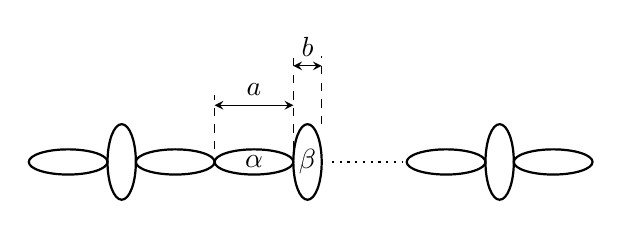
\begin{tikzpicture}[>=stealth, thick, scale=1.0]
  % Top: chain of monomers (alpha = horizontal ellipse width a=1.0, beta = vertical ellipse width b=0.36)
  \draw[thick] (0.5, 0) ellipse (0.5 and 0.16);
  \draw[thick] (1.18, 0) ellipse (0.18 and 0.48);
  \draw[thick] (1.86, 0) ellipse (0.5 and 0.16);
  \draw[thick] (2.86, 0) ellipse (0.5 and 0.16);
  \node at (2.86, 0) {$\alpha$};
  \draw[thick] (3.54, 0) ellipse (0.18 and 0.48);
  \node at (3.54, 0) {$\beta$};

  \draw[dotted, thick] (3.85, 0) -- (4.75, 0);

  \draw[thick] (5.30, 0) ellipse (0.5 and 0.16);
  \draw[thick] (5.98, 0) ellipse (0.18 and 0.48);
  \draw[thick] (6.66, 0) ellipse (0.5 and 0.16);

  % Dimension arrows for a and b
  \draw[dashed, thin] (2.36, 0.16) -- (2.36, 0.85);
  \draw[dashed, thin] (3.36, 0.16) -- (3.36, 1.35);
  \draw[dashed, thin] (3.72, 0.48) -- (3.72, 1.35);

  \draw[<->, thin] (2.36, 0.72) -- (3.36, 0.72) node[midway, above] {$a$};
  \draw[<->, thin] (3.36, 1.22) -- (3.72, 1.22) node[midway, above] {$b$};
\end{tikzpicture}
\end{document}
